\chapter{Statistics}
\section{Modelling the Single Lepton Analysis}
\label{sec:inter_1lepton}
As described in the previous section, the core component of many statistical
interpretations is the construction of an appopriate likelihood function. The
likelihood must model all statistical and systematic effects and is thus highly
dependent on the experiment. The situation is considerably complicated when
shape information is included, for which relevant bin-to-bin correlations must
be included.

\subsection{Notation}
It will be helpful to define some notation. In the following, a subscript index
is assumed to run over the binned variable in the analysis (i.e. \STlep). All
nuisance parameters are written as $\nu^{(i)}$ where the superscript index is
taken to run over some set of systematic uncertainties
(e.g. $\nu^{\textrm{jes}}$ might represent the \acl{JES} uncertainty). Certain
variables $x$ are known to have a functional dependence on a given nuisance
parameter and are written $x(\nu)$. The nominal value of this variable, being
that which is measured in \ac{MC} or in real data is denoted $\bar{x}$.

\subsection{The Likelihood Function}
In constructing the likelihood, we start by writing down the number of events
expected for each bin (assigned the index $i=0,1,2...$):
\begin{equation*}
\NExpi = \NSigi(\mu, \nu^{(j)}) +
\NBkgi(\nu^{(k)}),
\end{equation*}
where \NSigi is the expected signal yield for a chosen signal model and \NBkgi
is the data-driven background prediction. As can be seen, the signal yield is a
function of the \ac{poi} -- the signal strength -- and some number of nuisance
parameters where the index $j$ will run over a set of systematic uncertainties
relevant to the signal yield. Ignoring signal contamination effects (which will
be discussed later), the bacground yield depends only on the nuisance parameters
$\nu^{(k)}$ where $k$ is taken to run over the set of systematic uncertainties
relevant to the background prediction.

Without giving an explicit functional form for the signal yield and background
prediction, the form of the likelihood function may be constructed. The
likelihood must include:
\begin{enumerate}
\item Statistical terms representing the likelihood of observing the given
  number of events given a certain expectation for the signal and background
  yields.
\item Terms providing prior constraints on the various nuisance
  parameters. Certain uncertainties are statistical in nature and thus,
  independent nuisance parameters are assigned per bin along with a corresponding
  prior pdf. In other cases, the underlying systematic variation is considered
  to have a 100\% correlated effect across the bins. In these cases, a single
  nuisance parameter and prior pdf is assigned.
\end{enumerate}

The form of the likelihood is as follows,
\begin{equation*}
\mathcal{L} = \prod_i \Poisson(\NExpi ; \NObsi)
\prod_{\alpha \in \Theta}  X_\alpha(\nu^{(\alpha)}),
\end{equation*}
where:
\begin{itemize}
\item $\mathcal{P}(\mu;x)$ denotes a Poisson distribution with mean $\mu$ and value
$x$ and
\item the $X_\alpha(\nu^{(\alpha)})$ represent some prior pdf associated with
  each systematic $\alpha$.
\end{itemize}

\subsection{The Signal Yield}
The signal yield per bin is constructed as follows:
\begin{equation*}
\NSigi = \mu \times \epsilon_i(\nu^{(\alpha)}) \times \sigma \times L \times \nu^{\textrm{lumi}},
\end{equation*}
with:
\begin{itemize}
\item $\epsilon_i(\nu^{(\alpha)})$ is the efficiency of the $i$th bin assumed to be
  dependent on a set of nuisance parameters $\nu^{(\alpha)}$;
\item $\sigma$ the cross-section of the signal model being considered;
\item $L$ the integrated luminosity and
\item $\nu^{\textrm{lumi}}$ the nuisance parameter associated with uncertainty in the
estimate of the integrated luminosity.
\end{itemize}
The \ac{poi}, $\mu$ then represents the ratio of the upper limit on the
cross-section to the chosen model cross-section, $\sigma$. Note that for the
simplified model limits, the parameter $\sigma$ was set to 1 and therefore the
\ac{poi} itself represents a cross-section.

\subsection{Background Prediction}
The background prediction per bin is then written as
\begin{equation*}
\NBkgi = \RCSi(\nu_i^{(\alpha)}, \nu^{(\beta)}) \times \NControli(\nu_i^{(\gamma)}),
\end{equation*}
where:
\begin{itemize}
\item \RCSi is the translation ratio as defined in \eqn~\ref{eqn:susysearch_RCS};
\item the nuisance parameters $\nu_i^{(\alpha)}$ and $\nu_i^{\gamma}$ represent
  statistical uncertainties uncorrelated between the bins;
\item the nuisance parameters $\nu_i^{(\beta)}$ represent systematic
  uncertainties assumed to be 100\% correlated across the bins and
\item \NControli the observed number of events in the control region
(\LPcontrol)
\end{itemize}

\subsection{Parameterising Systematic Uncertainties}
In reality, it is almost always impossible to obtain a full functional form for
a variable $x$ (e.g. \RCSi, \NControli) in terms of a set of nuisance parameters
$\nu^{(\alpha)}$. Writing the Taylor expansion of $x(\nu^{(\alpha)})$ for two terms to
second order,
\begin{align*}
 x(\nu^{(A)}, \nu^{(B)})\bigg|_{\substack{\nu^{(A)} = a\\ \nu^{(B)} = b}} \approx
x(a,b) +
(\nu^{(A)} - a)\left.\frac{\partial x}{\partial\nu^{(A)}}\right|_{\nu^{(A)}=a} +
(\nu^{(B)} - b)\left.\frac{\partial x}{\partial\nu^{(B)}}\right|_{\nu^{(B)}=b} +\\
\frac{1}{2!}\left[
(\nu^{(A)} - a)^2 \frac{\partial^2 x}{\partial \left(\nu^{(A)}\right)^2}
+ (\nu^{(B)} - b)^2 \frac{\partial^2 x}{\partial \left(\nu^{(B)}\right)^2}
+ 2(\nu^{(A)} - a)(\nu^{(B)} - b)\frac{\partial^2 x}{\partial
  \nu^{(A)}\partial\nu^{(B)}}
\right].
\end{align*}
Assuming the expansion is performed with respect to the mean of x, $\bar{x}$,
the values of $a$ and $b$ are seen to be the mean values of the corresponding nuisance
parameters. For small deviations from the mean,
\begin{equation*}
 (\nu^{(A)} - a) \sim (\nu^{(B)} - b) \sim \epsilon \sim 0,
\end{equation*}
and ignoring terms $O(\epsilon^2)$,

\begin{equation}
\label{eqn:stats:taylor}
x(\nu^{(A)}, \nu^{(B)}) \approx \bar{x} +
(\nu^{(A)} - a)\left.\frac{\partial x}{\partial\nu^{(A)}}\right|_{\nu^{(A)}=a} +
(\nu^{(B)} - b)\left.\frac{\partial x}{\partial\nu^{(B)}}\right|_{\nu^{(B)}=b}.
\end{equation}
Since the derivatives in \eqn~\ref{eqn:stats:taylor} will in practice be
derived from some finite variation of the underlying quantity associated with
each nuisance parameter, the infinitessimal derivatives must be replaced by
finite changes. It is also sensible to set $a=b=0$,
\begin{equation}
\label{eqn:stats:taylor2}
x(\nu^{(A)}, \nu^{(B)}) \approx \bar{x} +
\nu^{(A)}\frac{\Delta x}{\Delta\nu^{(A)}} +
\nu^{(B)}\frac{\Delta x}{\Delta\nu^{(B)}}.
\end{equation}
Since the value of $x$ is often associated with a physical quantity such as an
efficiency or an event yield, it is desirable to constrain it to positive
values. This can be achieved providing the range of each nuisance parameter is
set such that,
\begin{equation*}
\nu^{(\alpha)}\times\frac{\Delta x}{\Delta \nu^{(\alpha)}} < \bar{x}.
\end{equation*}

The previous derivation can be simply extended two $N > 2$ nuisance
parameters. Generalising and rewriting \eqn~\ref{eqn:stats:taylor2},
\begin{eqnarray*}
x(\nu^{(A)}, \nu^{(B)}, \ldots) &\approx& \bar{x} +
\nu^{(A)}\frac{\Delta x}{\Delta\nu^{(A)}} +
\nu^{(B)}\frac{\Delta x}{\Delta\nu^{(B)}} + \ldots \\
&\approx& \frac{1}{\bar{x}^{N-1}} \left\{ \bar{x}^N +
\bar{x}^{N-1} \nu^{(A)}\frac{\Delta x}{\Delta\nu^{(A)}} +
\bar{x}^{N-1} \nu^{(B)}\frac{\Delta x}{\Delta\nu^{(B)}} + \ldots \right\}.
\end{eqnarray*}
If we attempt to rewrite as a product,
\begin{eqnarray*}
\prod_{j=A, B, \ldots} \left(\bar{x} + \frac{\Delta x}{\Delta\nu^{(\alpha)}}\right) &=&
\bar{x}^N + \bar{x}^{N-1} \sum_{j=A, B, \ldots} \nu^{(\alpha)}\frac{\Delta x}{\Delta \nu^{(\alpha)}} \\
&&+ \bar{x}^{N-2}\sum_{j=A, B, \ldots} \sum_{k=A, B, \ldots} \nu^{(\alpha)}\nu^{(\beta)}\frac{\Delta x}{\Delta
  \nu^{(\alpha)}}\frac{\Delta x}{\Delta \nu^{(\beta)}} \\
&&+ \ldots +O(\nu^N).
\end{eqnarray*}
Ignoring terms greater than $O(\nu^2)$,
\begin{eqnarray*}
\prod_{j=A, B, \ldots} \left(\bar{x} + \frac{\Delta x}{\Delta\nu^{(\alpha)}}\right) &\approx&
\bar{x}^N + \bar{x}^{N-1} \sum_{j=A, B, \ldots} \nu^{(\alpha)}\frac{\Delta x}{\Delta
  \nu^{(\alpha)}} \\
&\approx& \bar{x}^{N-1} x(\nu^{(A)}, \nu^{(B)}, \ldots),
\end{eqnarray*}
and therefore
\begin{equation}
\label{eqn:stats:systderiv}
x(\nu^{(A)}, \nu^{(B)}, \ldots) \approx \frac{1}{\bar{x}^{N-1}} \prod_{j = A, B,
  \ldots} \left(\bar{x} + \frac{\Delta x}{\Delta\nu^{(\alpha)}}\right) \approx
\bar{x} \prod_{j = A, B,
  \ldots} \frac{1}{\bar{x}}\left(\bar{x} + \frac{\Delta x}{\Delta\nu^{(\alpha)}}\right).
\end{equation}

Using \eqn~\ref{eqn:stats:systderiv}, the signal yield can be rewritten as follows:
\begin{equation*}
\NSigi = \mu \times \bar{\epsilon}_i \times \prod_{j}\left(\frac{\bar{\epsilon}_i
    + \nu^{(\alpha)}\frac{\Delta\epsilon_i}{\Delta\nu^{(\alpha)}}}{\bar{\epsilon}_i}\right) \sigma \times L \times \nu^{\textrm{lumi}},
\end{equation*}
and the background prediction,
\begin{equation*}
\NBkgi = \RbarCS_i \times \prod_{j}\left( \frac{\RbarCS_i
    + \nu^{(\alpha)}\frac{\Delta\RCSi}{\Delta\nu^{(\alpha)}}}{\RbarCS_i}\right)
\times \NbarControl_i \times \prod_{k}\left( \frac{\NbarControl_i
    + \nu^{(\alpha)}\frac{\Delta\NControli}{\Delta\nu^{(\beta)}}}{\NbarControl_i}\right).
\end{equation*}

\subsection{Nuisance Parameters}
The nuisance parameters incorporated in the model described thus far are of two
types.
\begin{enumerate}
\item Statistical uncertainties assumed to be uncorrelated across analysis
  bins. This includes uncertainties arising from the limited statistical
  precision of the \ac{MC} sample and limited data in the control region.
\item Systematic uncertainties arising from detector artefacts or theoretical
  uncertainties such as \ac{JES}, standard model cross-section
  calculations and the luminosity measurement~\cite{cms_lumi_measurement}.
\end{enumerate}
For uncertainties of the first kind, independent nuisance paramters must be
included for each analysis bin. For uncertainties of the second kind, a single
nuisance parameter will be included for all bins -- giving the desired
correlation. A full list of the nuisance parameters used is shown in
Table~\ref{tbl:inter_systematic_parameters}. For the work presented here,
Gaussian prior distributions have been used for all nuisance parameters.

\ctable[
cap=Nuisance parameters included in the single lepton likelihood function,
caption=Summary of nuisance parameters included in the single lepton likelihood function.,
mincapwidth=0.5\textwidth,
label=tbl:inter_systematic_parameters,
pos=h,
doinside=\scriptsize
]{lccccc}{
\tnote[a]{Muon channel only}
\tnote[b]{Electron channel only}

\tnote[c]{In the electron channel, the use of \ac{MC} templates in the QCD
  background estimate introduces a dependence on the \ac{JES}. Whilst the
  ability to include these correlations was added to the statistics package, it
  was not used in the results shown.}

}{\FL
Uncertainty                        & Correlated & \NSigi     & \RCSi      & \NControli & Nuisance Parameters\ML
%
Luminosity                         & \checkmark & \checkmark &            &            & $\nu^{\textrm{lumi}}$\NN
\acf{JES}                          & \checkmark & \checkmark & \checkmark & \tmark[c]  & $\nu^{\textrm{jes}}$\NN
\MET Resolution                    & \checkmark & \checkmark & \checkmark & \tmark[c]  & $\nu^{\textrm{metres}}$\NN
\PW/\Ptop\APtop Ratio              & \checkmark &            & \checkmark &            & $\nu^{W\Ptop\APtop}$\NN
\PW Polarisation                   & \checkmark &            & \checkmark &            & $\nu^{\textrm{\PW pol}}$\NN
Muon Momentum Scale\tmark[a]       & \checkmark &            & \checkmark &            & $\nu^{\textrm{lep}}$\NN
Limited \ac{MC} Statistics         &            &            & \checkmark &            & $\nu^{\textrm{MC}}_i$\NN
Limited Data Statistics            &            &            &            & \checkmark & $\nu^{\textrm{data}}_i$\NN
Signal Contamination               &            &            &            & \checkmark & $\nu^{\textrm{sig cont}}_i$\NN
\ac{PDF} Uncertainties             & \checkmark & \checkmark &            &            & $\nu^{\textrm{pdf}}_i$\NN
QCD Background Prediction\tmark[b] &            &            &            & \checkmark & $\nu^{\textrm{qcd}}_i$\LL
}

An additional nuisance parameter reflecting signal contamination in the control
region requires a more careful choice of likelihood terms. This is described in
the next section.

\subsection{Signal Contamination}
It can be seen in \fig~\ref{fig:susy_lp} that the region \LPcontrol may have a
substantial component of \ac{SUSY} events depending on the particular model
under consideration. Signal contamination increases \NControl leading to an
overprediction of \NBkg. To account for this, the \NBkgi term is modifed to
reflect the assumption that some fraction of the yield \NControli will be due to
\ac{SUSY} contamination. Rewriting,

\begin{equation}
\label{eqn:bgprediction}
\NBkgi(\mu, \nu^{(\alpha)}) = \RbarCS_i \times \prod_{j}\left( \frac{\RbarCS_i
    + \nu^{(\alpha)}\frac{\Delta\RCSi}{\Delta\nu^{(\alpha)}}}{\RbarCS_i}\right)
\times \NbarControl_i \times f^{\textrm{SM}}_i(\mu) \times \prod_{k}\left( \frac{\NbarControl_i
    +
    \nu^{(\alpha)}\frac{\Delta\NControli}{\Delta\nu^{(\beta)}}}{\NbarControl_i}\right),
\end{equation}
where $f^{\textrm{SM}}_i$ represents the fraction of \NControli expected to be
\ac{SM} events given the current signal hypothesis i.e.
\begin{equation*}
f^{\textrm{SM}}_i(\mu) = \frac{\NSMi}{\NSMi + \NSUSYi(\mu)}.
\end{equation*}
The expected number of \ac{SUSY} events $\NSUSYi =
\mu\times\epsilon^{\textrm{control}}_i\times\sigma\times L$ where
$\epsilon^{\textrm{control}}_i$ is the efficiency calculated for \ac{SUSY}
events entering the \LPcontrol control region. To reflect these constraints, we
set up an appropriate prior distribution,
\begin{equation*}
X(\nu^{\textrm{SM}}) = \Gauss \left( \frac{\NSMi}{\NSMi + \mu\times\epsilon_i^{\textrm{control}}\times\sigma\times L}
; \nu^{\textrm{SM}} \right),
\end{equation*}
and $f^{\textrm{SM}}_i \equiv \nu^{\textrm{SM}}_i$. Calculating the expected value of the nuisance parameter,
\begin{eqnarray}
\label{eqn:fSMideal}
<f^{\textrm{SM}}_i> &=& \frac{\NSMi}{\NSMi + \mu\NSUSYi}\nonumber \\
                   &=& \frac{1}{1 + \mu\frac{\NSUSYi}{\NSMi}}.
\end{eqnarray}
Technical problems associated with adding a functional dependence on the
\ac{poi} $\mu$ to the mean of the prior distribution necessitated a slightly
altered formulation. As will be shown, this formulation is approximately
equivalent given certain assumptions about the range of $\mu$ and the degree of
signal contamination. The prior distribution included in \likelihood is
rewritten as
\begin{equation*}
X(\nu^{\textrm{SM}}_i) = \Gauss \left( \frac{\NSMi}{\NSMi + \epsilon_i^{\textrm{control}}\times\sigma\times L}
; \nu^{\textrm{SM}}_i \right).
\end{equation*}
The term included in the background prediction (\eqn~\ref{eqn:bgprediction})
is modified to
\begin{equation*}
f^{\textrm{SM}}_i = 1 - \mu \times \left(1- \nu^{\textrm{SM}}_i\right).
\end{equation*}
It can be seen that for $\mu=0$, $f^{\textrm{SM}}_i=1$ and for $\mu=1$,
$f^{\textrm{SM}}_i=\nu^{\textrm{SM}}_i$ as required. It will now be shown that
for a suitable range of $\mu$ and for small values of $\NSUSYi/\NControli$, the
expectation value of $f^{\textrm{SM}}_i$ will be equivalent to
\eqn~\ref{eqn:fSMideal}:
\begin{eqnarray*}
<f^{\textrm{SM}}_i> &=& 1 - \mu \times \left(1-<\nu^{\textrm{SM}}>\right) \\
                  &=& 1 - \mu  + \mu\frac{\NSMi}{\NSMi + \NSUSYi} \\
                  &=& \frac{(1-\mu)\left(\NSMi + \NSUSYi\right) + \mu\NSMi}{\NSMi + \NSUSYi} \\
                  &=& \frac{\NSMi + (1 - \mu)\NSUSYi}{\NSMi + \NSUSYi} \\
                  &=& \frac{\NSMi \left( 1 + (1-\mu)\frac{\NSUSYi}{\NSMi}\right)}{\NSMi + \NSUSYi} \\
                  &=& \frac{\NSMi}{\left(\NSMi +\NSUSYi\right)\left( 1 + (1 - \mu)\frac{\NSUSYi}{\NSMi}\right)^{-1}} \\
                  &\approx& \frac{\NSMi}{\left(\NSMi +\NSUSYi\right)\left( 1 - (1-\mu)\frac{\NSUSYi}{\NSMi}\right)} \\
                  &=& \frac{\NSMi}{\NSMi + \mu\NSUSYi - (1-\mu)\frac{\NSUSYi^2}{\NSMi}}\\
                  &=& \frac{1}{1 + \mu\frac{\NSUSYi}{\NSMi} - (1-\mu)\left(\frac{\NSUSYi}{\NSMi}\right)^2} \\
                  &\approx& \frac{1}{1 + \mu\frac{\NSUSYi}{\NSMi}}.
\end{eqnarray*}

\subsection{Uncertainties on \texorpdfstring{\NControli}{NControli}}
The dominant systematic uncertainty relating to the \LPcontrol region yield
arises from the limited statistics of the sample. This is especially true at
high \STlep. Accordingly, a nuisance parameter is added to the likelihood and
assigned a Gaussian prior with a width derived assuming a Poisson error on the
\NControli yield.

An additional complication arises in the case of the electron channel where the
\LPcontrol region has a non-negligible component of \ac{QCD} multijet
events. These are unreliably modelled by event generators and thus not included
in the calculation of \RCSi. This additional contribution to \NControli would
again lead to an overprediction of the background. To correct this, an
additional factor is included in Equation~\ref{eqn:bgprediction},
$f^{\textrm{ewk}}_i$ derived from the results of the \ac{QCD} fit detailed in
\sec~\ref{sec:susy_electron_bgpredict}. The error derived from the fit
procedure is modelled as a Gaussian prior on an additional nuisance parameter
$\nu^{\textrm{QCD}}_i$. It has been assumed, and confirmed by the results of the
fit in data that the region \LPsignal is \ac{QCD} free.

The uncertainty included via the prior distribution of $\nu^{\textrm{QCD}}$ was
the quadrature sum of the statistical error from the fitting procedure and an
uncertainty accounting for the limited generator statistics used to construct
the fit templates. Additional errors coming from the \ac{JES} uncertainty and
missing energy resolution were found to be small. Proper inclusion of these into
the likelihood would need to ensure correlation with the nuisance parameters
representing these uncertainties. The relevant terms were set up but not
included in the final calculations. The contribution is seen to be small and
unnecessary complication of the likelihood function tends to increase the
processing time, especially when running a large number of toy experiments.

\section{Validation Plots}
\label{sec:app_inter_validation}
Additional validation plots for the \ac{CMSSM} point $(\Mzero, \Mhalf) = (80,
240)$ are shown in \figs~\ref{fig:app_pl}~and~\ref{fig:app_cls}. This is a
point far below the edge of the excluded region. They are otherwise identical to
the plots shown in \sec~\ref{sec:inter_validation}.

% A comparison of the \Ttwott upper limit with similar analyses at \ac{CMS} is
% shown in \fig~\ref{fig:lp_ls_t2tt}. Note that this limit does not include any
% uncertainties on the signal efficiencies.

\begin{figure}[h!]
\centering
\subfloat[]{\label{fig:inter_pl_80_240_syst}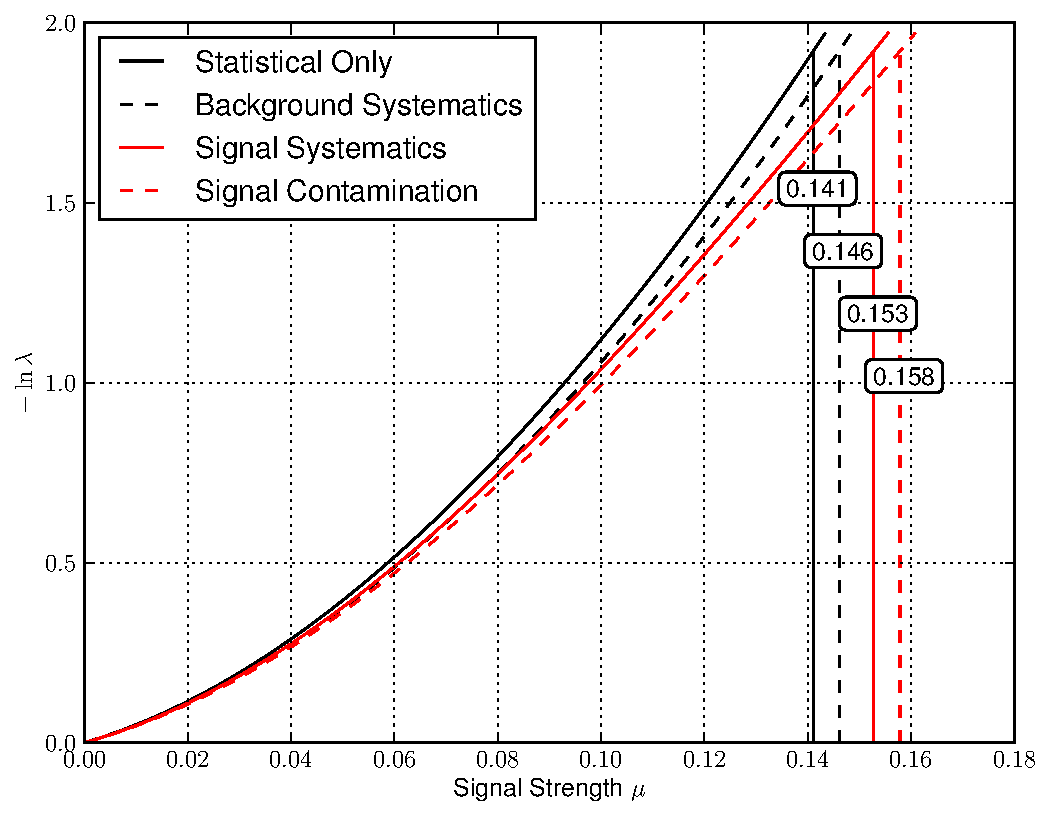
\includegraphics[width=0.47\textwidth]{fig/pl_systematics_80_240}}\quad
\subfloat[]{\label{fig:inter_pl_80_240_muon}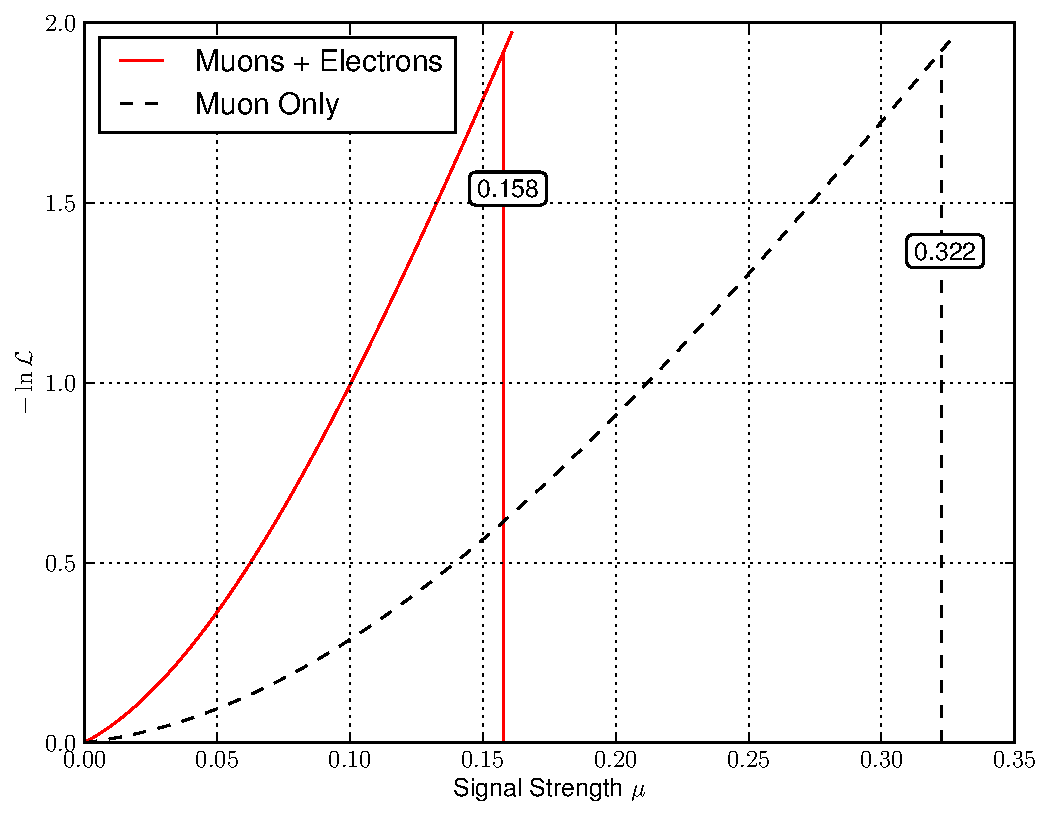
\includegraphics[width=0.47\textwidth]{fig/pl_muon_80_240}}
\caption{Comparison of the shape of the profile likelihood function with
  different systematic effects included at the \ac{CMSSM} point $(\Mzero, Mhalf)
  = (80, 240)$}
\label{fig:app_pl}
\end{figure}


\begin{figure}[h!]
\centering
\subfloat[Statistical Uncertainties Only]{
  \label{fig:inter_cls_80_240_1}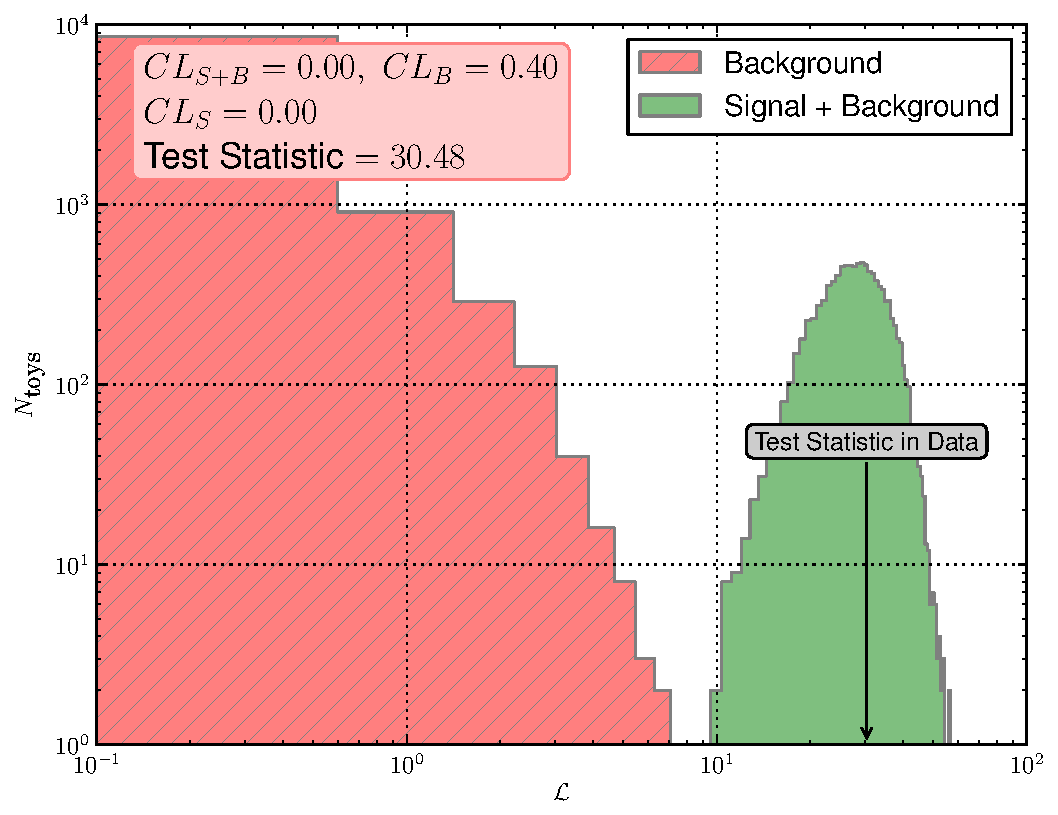
\includegraphics[width=0.47\textwidth]{fig/exp_muon_electron_80_240_bgsysts_no_sigsysts_no_sigcon_no}}\quad
\subfloat[Background Uncertainties]{
  \label{fig:inter_cls_80_240_2}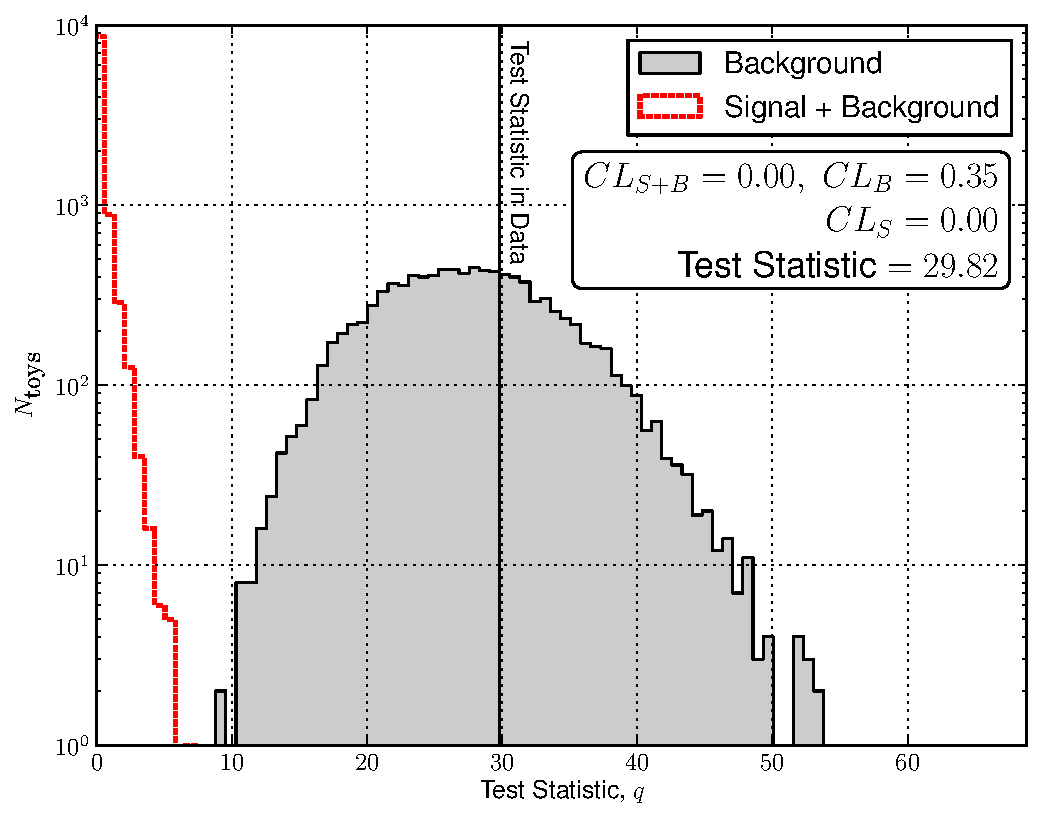
\includegraphics[width=0.47\textwidth]{fig/exp_muon_electron_80_240_bgsysts_yes_sigsysts_no_sigcon_no}}\\
\subfloat[Signal Uncertainties]{
  \label{fig:inter_cls_80_240_3}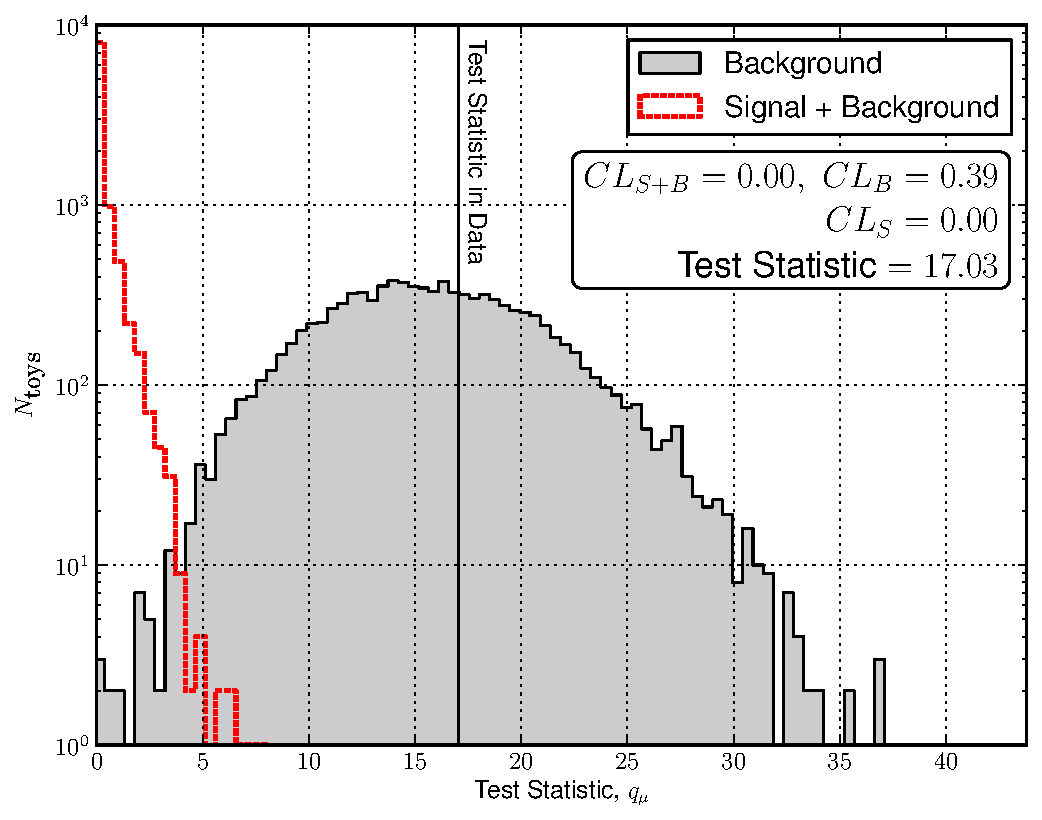
\includegraphics[width=0.47\textwidth]{fig/exp_muon_electron_80_240_bgsysts_yes_sigsysts_yes_sigcon_no}}\quad
\subfloat[Signal Contamination]{
  \label{fig:inter_cls_80_240_4}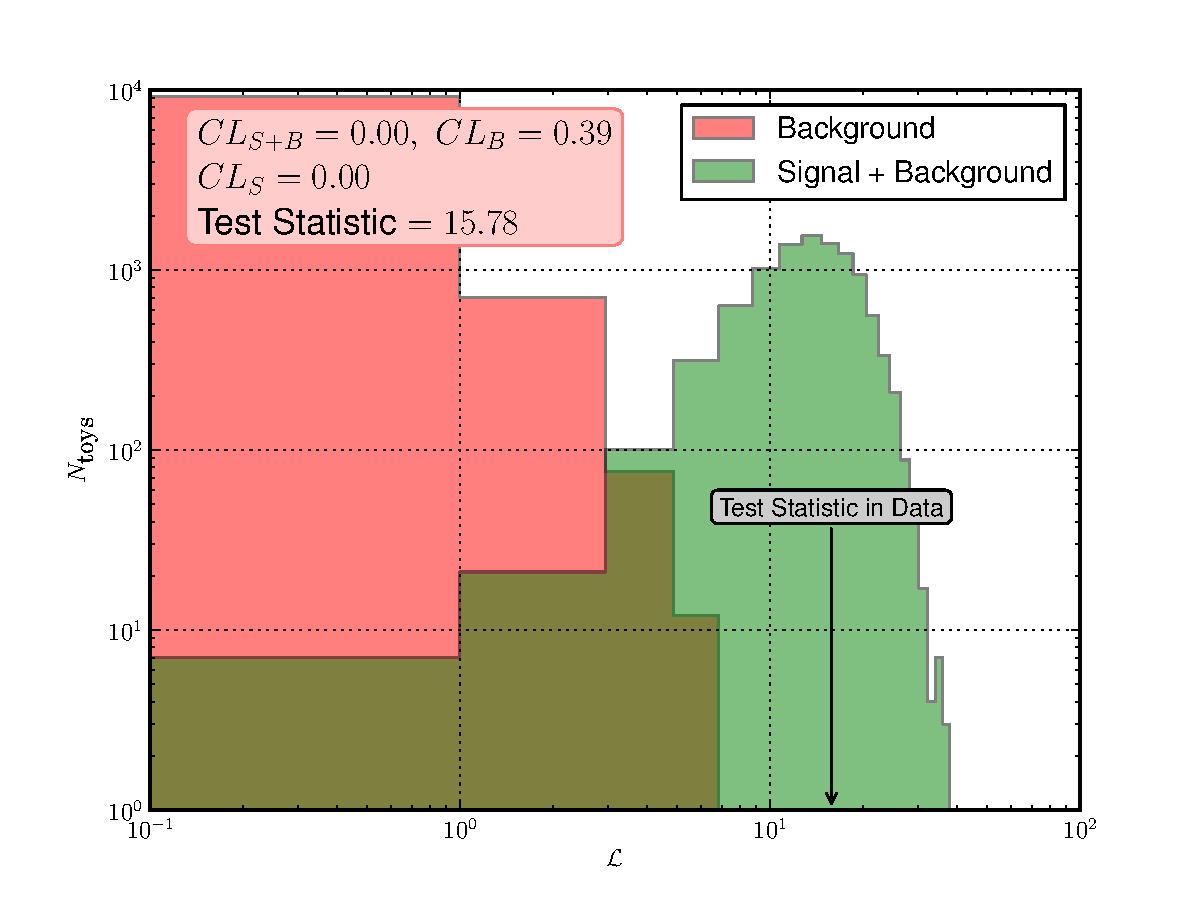
\includegraphics[width=0.47\textwidth]{fig/exp_muon_electron_80_240_bgsysts_yes_sigsysts_yes_sigcon_yes}}\\
\subfloat[Muon Channel Only]{
  \label{fig:inter_cls_80_240_5}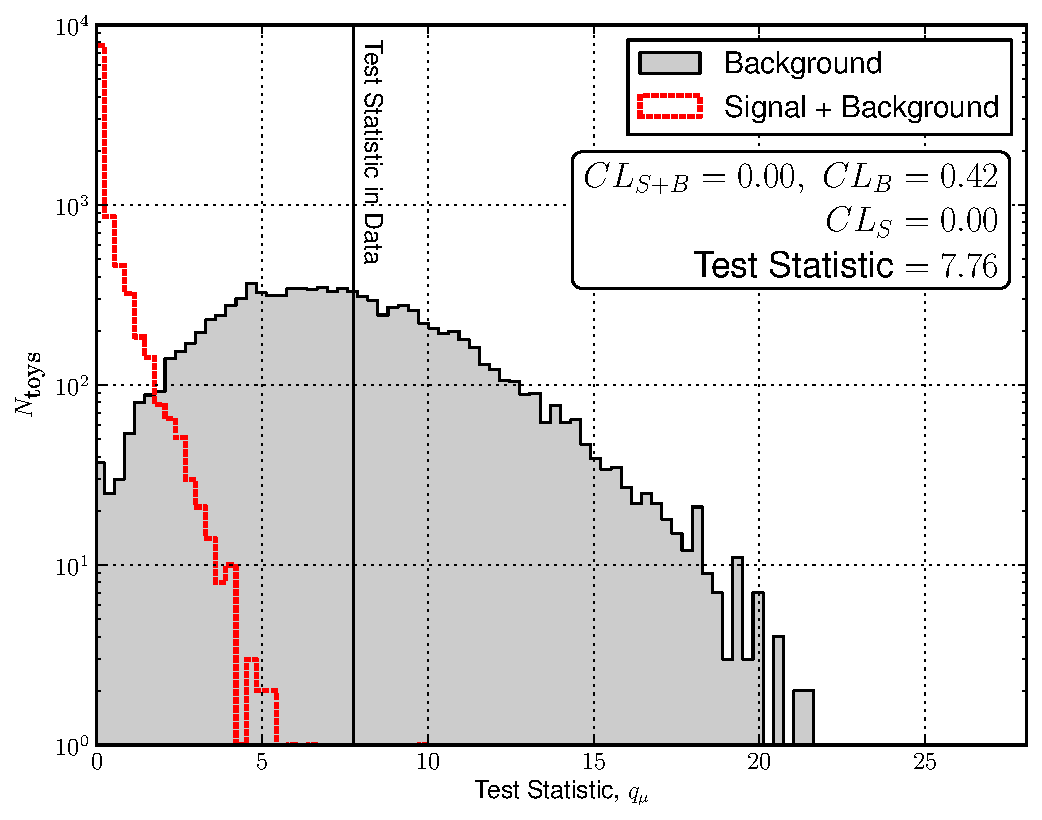
\includegraphics[width=0.47\textwidth]{fig/exp_muon_80_240_bgsysts_yes_sigsysts_yes_sigcon_yes}}
\caption[Distribution of the profile likelihood ratio test statistic for null
and alternate hypotheses with different systematic effects
included.]{Distribution of the profile likelihood ratio test statistic for null
  and alternate hypotheses with different systematic effects included. These
  distributions have been made for the \ac{CMSSM} point $(\Mzero, \Mhalf) = (80,
  240)$. The values of \CLb, \CLspb and \CLs are also shown.}
\label{fig:app_cls}
\end{figure}

% \begin{figure}[h!]
% 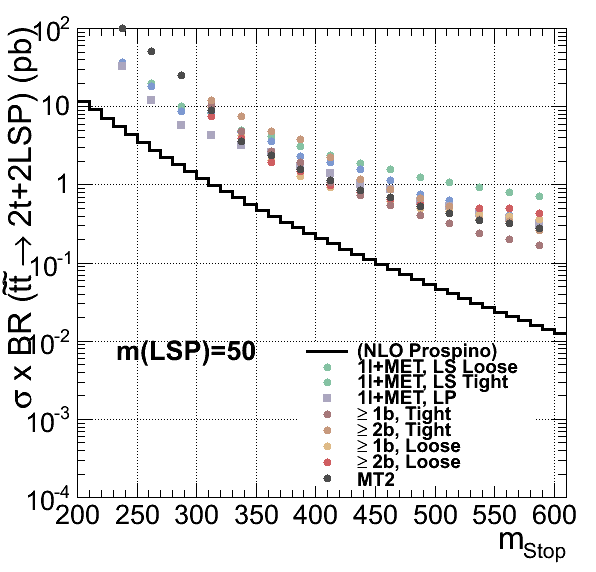
\includegraphics[width=0.6\textwidth]{fig/StopResult}
% \caption{Comparison of the upper limits set by a number of analyses in the
%   \Ttwott simplified model for $\Mlsp = \unit{50}{\GeV}$ . The \LP result is
%   shown as grey squares. The \ac{QCD} \ac{NLO} cross-section as calculated by
%   \prospino is also shown.}
% \label{fig:lp_ls_t2tt}
% \end{figure}